\documentclass[11pt]{article}

\usepackage{amsfonts}
\usepackage{enumitem}
\usepackage{graphicx}

\title{6.047 Problem Set 3 Writeup}
\author{Matthew Feng}
\date{\today}

\begin{document}
\maketitle

\section{Gibbs sampling for motif discovery}
\subsection*{(a) Gibbs sampling}
My implementation of Gibbs sampling attempts to introduce
randomization in as many locations as possible, with the
goal to avoid becoming trapped in local maxima. As such,
the sequence that is excluded is selected, but in
a randomly shuffled order, so that every sequence is
selected at the same frequency, but with randomization.
Additionally, I incorporated the background probabilities of
the bases as a ``score correction'', dividing the probability
of observing motifs by the probability of the motif given the
background distribution, to avoid focusing
in on motifs that are simply more abundant, rather than
more informative.

\subsection*{(b) Test cases}

The most probable PWM for each of the datasets can be found in
the {\tt pwms/} folder. See Figures 1, 2, 3 and 4 for the most
probable PWMs as sequence logos.

\begin{figure}
\noindent\makebox[\textwidth]{
    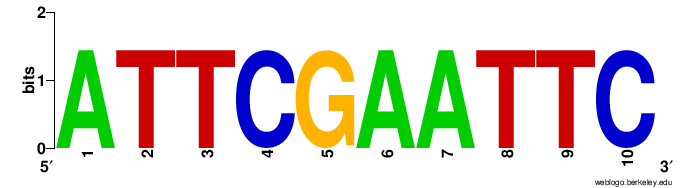
\includegraphics[width=0.5\paperwidth]{../problems/problem1/logos/data1logo.png}
}
\caption{Most probable motif in {\tt data1.txt}.}
\end{figure}

\begin{figure}
\noindent\makebox[\textwidth]{
    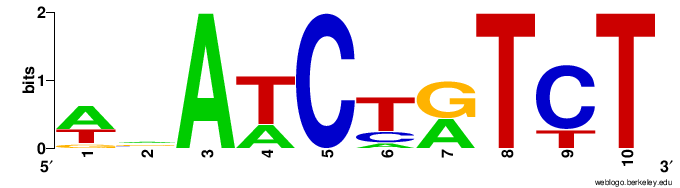
\includegraphics[width=0.5\paperwidth]{../problems/problem1/logos/data2logo.png}
}
\caption{Most probable motif in {\tt data2.txt}.}
\end{figure}

\begin{figure}
\noindent\makebox[\textwidth]{
    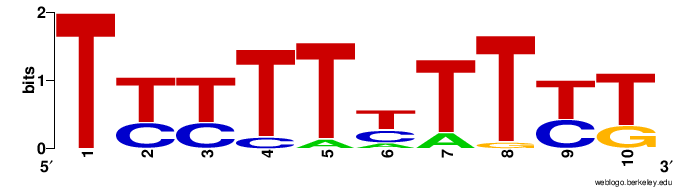
\includegraphics[width=0.5\paperwidth]{../problems/problem1/logos/data3logo.png}
}
\caption{Most probable motif in {\tt data3.txt}.}
\end{figure}

\begin{figure}
\noindent\makebox[\textwidth]{
    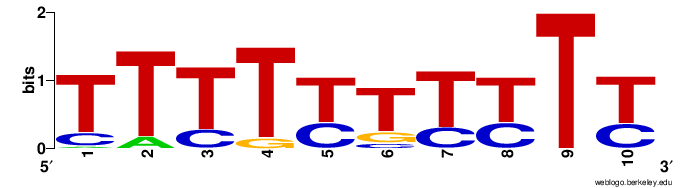
\includegraphics[width=0.5\paperwidth]{../problems/problem1/logos/data4logo.png}
}
\caption{Most probable motif in {\tt data4.txt}.}
\end{figure}

\section{Evolutionary signatures of motifs}
\subsection*{(a) Frequency vs. Conservation}
See {\tt kmers.py} for determining $k$-mer frequency and
conservation ratio.\\
See {\tt motif\_match.py} for matching potential $k$-mer
motifs against known motifs (i.e. testing for viability
of the algorithm).\\
See {\tt freq\_vs\_conserved.txt} for the top 50 most
frequently occuring $k$-mers and the top 50 most
highly conserved $k$-mers.

\subsection*{(b) Validation}
Simply counting the frequency of a $6$-mer as a motif has its
bias in that the more frequently appearing nucleotides will
be overrepresented; in other words, common sequences that
do not have particular meaning will tend to be the most
frequent $k$-mers.

As such, we should use the most percentage conserved motifs
instead, as conservation usually implies that certain sequences
have been important throughout evolution.

From the most conserved $6$-mers, we identified the following
motifs:
\begin{enumerate}[noitemsep]
\item {\tt CACGTG} $\rightarrow$ PHO4
\item {\tt ACGCGT} $\rightarrow$ SWI6
\item {\tt GATGAG} $\rightarrow$ ESR1

\end{enumerate}

\section{RNA secondary structure}
\subsection*{(a) Nussinov algorithm}
See {\tt nussinov.py} for the implementation details. The
program uses dynamic programming using a bottom-up
approach for greater efficiency.

\subsection*{(b)}
The average Nussinov score across $1000$ randomly generated
RNA sequences is $-44.155$.

\subsection*{(c)}
As length increases, the score decreases (i.e. more pairings).\\

\noindent See Figure 5 for reference.

\begin{figure}[h]
\noindent\makebox[\textwidth]{
    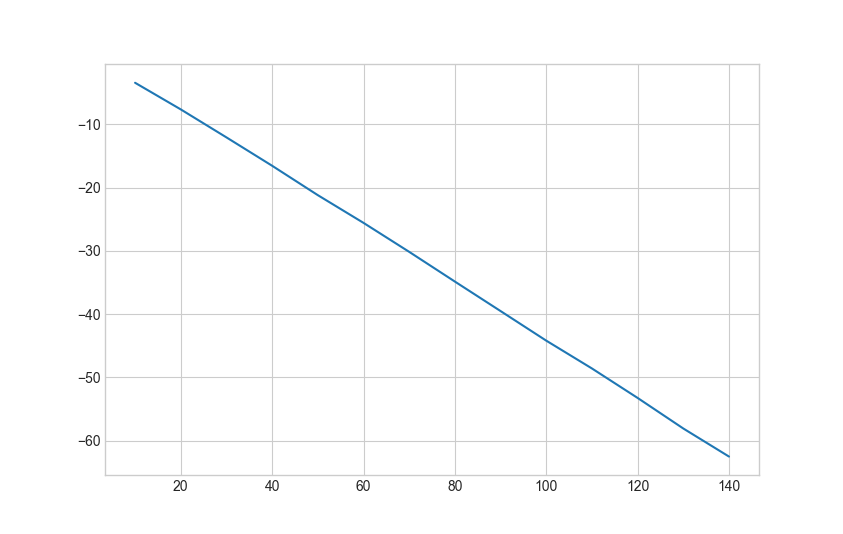
\includegraphics[width=0.5\paperwidth]{../problems/problem3/seqlength_to_score.png}
}
\caption{As sequence length increases, the score decreases (i.e. more
bases are paired). Sequence length is along the horizontal axis, while
the Nussinov score is along the vertical axis.}
\end{figure}

\subsection*{(d)}
As GC content approaches $0.5$, number of pairs decreases (i.e. score
becomes less negative), and then increases again (i.e. score becomes
more negative) as the GC content approaches $1.0$. The score function
is symmetric about GC content of 0.5 because as GC content decreases,
the number of A-U pairs is likely to increase, but when GC content
increases, the number of G-C pairs is likely to increases, either
of which compensates for the other.\\

\noindent See Figure 6 for reference.

\begin{figure}[h]
\noindent\makebox[\textwidth]{
    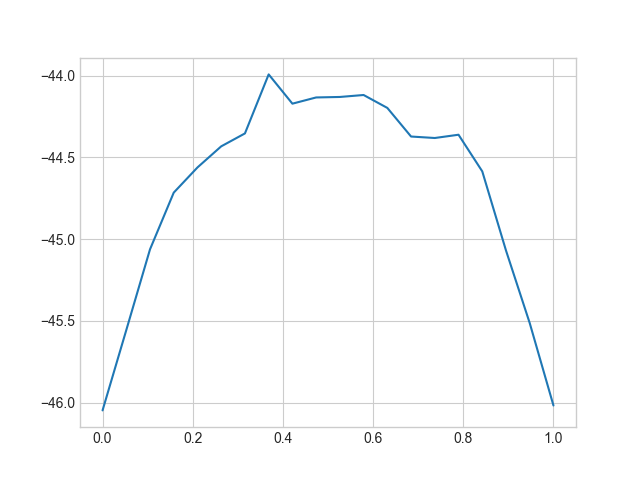
\includegraphics[width=0.5\paperwidth]{../problems/problem3/gccontent_vs_score.png}
}
\caption{As percentage of GC content increases, the score initially
increases, and then decreases after passing 50\%. The Nussinov
score is along the vertical axis, while the fraction of
GC content is along the horizontal axis.}
\end{figure}

\subsection*{(e)}

Since both length and percentage of GC content influence the 
score output by the Nussinov algorithm, it may be useful to
normalize the score (correct the score) by dividing by the length
and $\alpha\,+\,|0.5 - p|$, where $p$ is the percentage of GC content
and $\alpha$ is a hyperparameter to be tuned. The division essentially
``cancels out'' any effect of the length and percentage had in the
numerator.

\end{document}
